\documentclass[12pt]{article}

\usepackage{graphicx}
\usepackage{booktabs}
\usepackage{array}
\usepackage{url}
\usepackage{amsmath}
\usepackage{geometry}
\geometry{margin=1in}

\begin{document}

\title{Layout-Aware Text Column Detection and Reading-Order Recovery for Traditional Mongolian Historical Archives}

\author{\parbox{0.95\textwidth}{\centering Lanying Liang$^{1}$ \quad Yuefeng Liu$^{2,*}$\\[0.4em]\small $^{1}$Archives, Inner Mongolia University of Science and Technology,\\\small Baotou, 014010, Inner Mongolia, China\\\small $^{2}$School of Digital and Intelligent Industry (School of Cyber Science and Technology),\\\small Inner Mongolia University of Science and Technology, Baotou, 014010, Inner Mongolia, China\\\small *Corresponding author: liuyuefeng@imust.edu.cn; Lanying Liang: 389647973@qq.com}}
\date{}
\maketitle

\begin{abstract}
Traditional Mongolian historical archives pose a challenging page-level document analysis problem because the script is vertically written, cursive, low-resource, and frequently degraded by aging paper, ink variation, seals, scanning rotation, and heterogeneous archive sources. Since expert transcription of handwritten traditional Mongolian columns is expensive and currently unavailable, this work focuses on an upstream but essential stage for full-page archival OCR: text-column detection and reading-order recovery. We construct a page-level annotation protocol that records text-column bounding boxes, ignored noise regions, orientation metadata, and reading order. We compare classical rule-based extraction, YOLOv8n, and a COCO-pretrained Faster R-CNN MobileNet detector with a rotation-aware reading-order recovery strategy. On an independent 11-page test split, YOLOv8n improves the project-level IoU@0.5 F1 score from 0.507 to 0.820 and achieves 0.900 reading-order accuracy, while Faster R-CNN reaches 0.823 F1 after fine-tuning. We further provide a crop-export-ready interface that can connect detected columns to an OCR recognizer, while explicitly not reporting CER/WER because column-level expert transcripts are not yet available. The study therefore provides an initial pilot-scale, partially reproducible layout-analysis benchmark for subsequent traditional Mongolian archival OCR research, subject to archive-image access restrictions.
\end{abstract}

\noindent\textbf{Keywords:} Historical document analysis; Traditional Mongolian archives; Text column detection; Reading order recovery; Low-resource OCR preprocessing

\section{Introduction}
Full-page recognition of traditional Mongolian historical archives requires more than a recognizer trained on isolated text lines. The input pages often contain many vertical handwritten columns, irregular spacing, red seals, page borders, paper stains, and inconsistent scan orientations. If the text columns are not localized and ordered reliably, downstream OCR modules receive incomplete or misordered crops, making page-level transcription unreliable.

In the present stage, expert transcription of handwritten traditional Mongolian archive columns is not available. Rather than reporting unverifiable OCR accuracy, this paper focuses on the upstream page-layout problem that can be rigorously evaluated with bounding-box and reading-order annotations. This setting is practically important: page-level layout annotations are much cheaper to obtain than full textual transcription, and they form the necessary bridge between scanned archive images and later recognition modules.

Our contributions are threefold. First, we define a page-level annotation protocol for traditional Mongolian archives, including text-column boxes, ignore regions, orientations, and reading order. Second, we provide an initial low-resource benchmark of rule-based and learning-based column detection under a unified IoU@0.5 matching protocol. Third, we implement a crop-export-ready interface that exports oracle and automatically detected column crops, while clearly separating layout evaluation from future transcription-based OCR evaluation.


\begin{figure}[t]
\centering
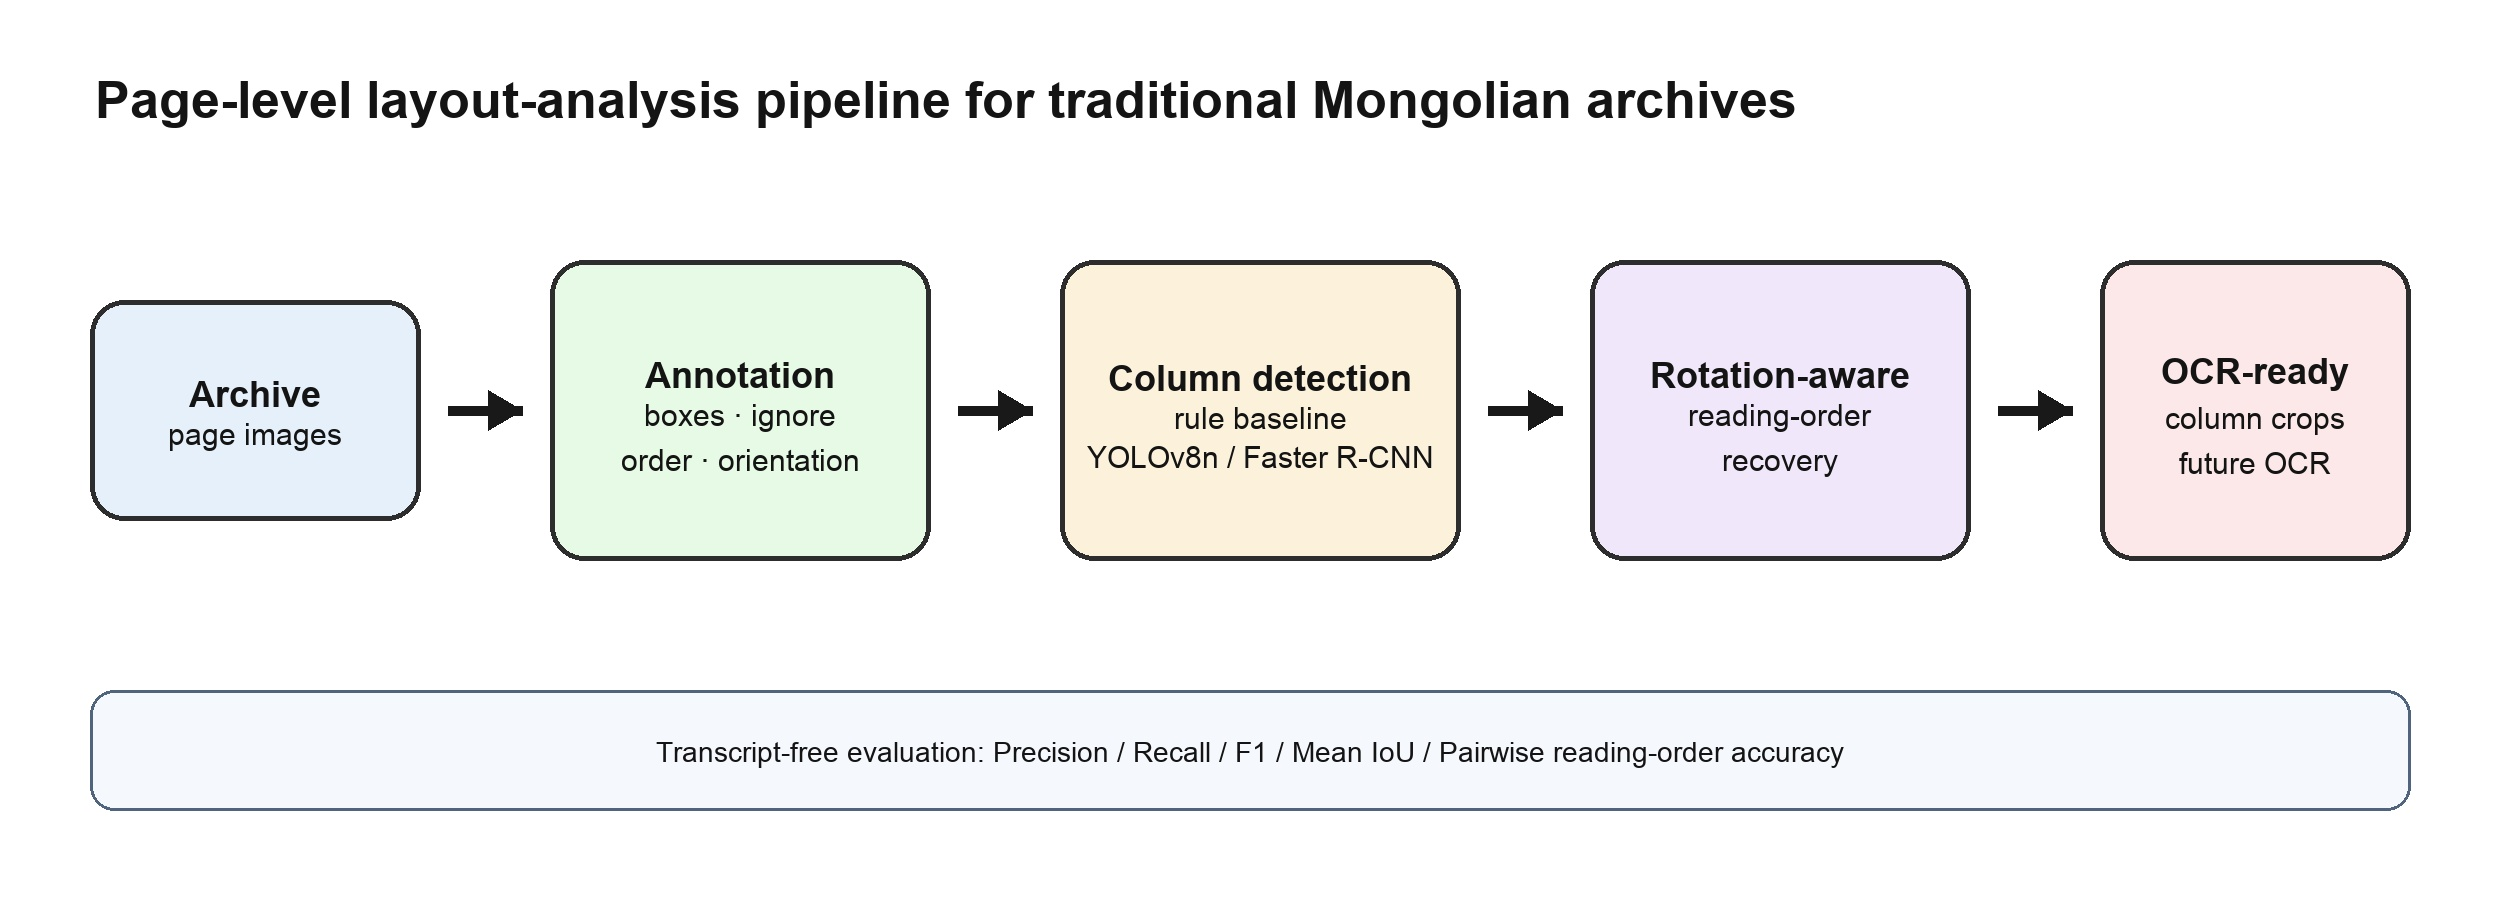
\includegraphics[width=\linewidth]{figures/page_layout_pipeline_overview.jpg}
\caption{Overview of the proposed page-level layout-analysis pipeline. The current study evaluates text-column detection and reading-order recovery without requiring expert text transcription.}
\label{fig:pipeline}
\end{figure}


\section{Related Work}
\subsection{Historical Document Layout Analysis}
Historical document image analysis has long treated segmentation as a prerequisite for reliable recognition. Likforman-Sulem et al.~\cite{likforman2007textline} review text-line segmentation methods for historical documents and emphasize that degradation, background noise, and handwriting variability make automatic page decomposition difficult. More recent dataset surveys also show that historical document collections vary widely in script, layout, degradation, and annotation granularity~\cite{nikolaidou2022survey}. For archival manuscripts, baseline and line detection datasets such as READ-BAD further highlight that realistic documents contain heterogeneous page layouts and challenging degradations~\cite{gruning2017readbad}. Traditional Mongolian recognition has also been studied at word or character level, including large online handwriting resources such as MOLHW~\cite{pan2023molhw}; however, page-level layout analysis for handwritten historical Mongolian archives remains underexplored. Our task is closely related to historical segmentation, but the target units are vertical traditional Mongolian text columns rather than horizontal baselines or printed regions.

\subsection{Learning-Based Document Layout Detection}
Large-scale document-layout datasets and toolkits have accelerated learning-based layout analysis. PubLayNet introduced a large automatically annotated dataset for scientific-document layout analysis~\cite{zhong2019publaynet}, while DocLayNet provided diverse human annotations for modern document layouts~\cite{pfitzmann2022doclaynet}. LayoutParser demonstrated how deep-learning layout models can be organized into reusable document-analysis pipelines~\cite{shen2021layoutparser}. Recent YOLO-style document-layout models further show that one-stage detectors remain competitive for document analysis when adapted to layout-specific scale and aspect-ratio variation~\cite{deng2023yolo, zhao2024doclayout}. These resources mainly focus on modern printed or PDF-derived documents, whereas our archive pages are handwritten, vertically arranged, and affected by scanning rotation and cultural-heritage degradation. We therefore train a lightweight detector on our own page-level annotations instead of relying on off-the-shelf layout categories.

\subsection{Reading Order and Recognition-Ready Preprocessing}
Reading-order recovery is necessary for transforming detected regions into structured text. Quir\'os and Vidal~\cite{quiros2022reading} show that handwritten document understanding still requires explicit ordering beyond line recognition. Historical OCR frameworks such as OCR-D also treat layout analysis, segmentation, and recognition as separate but connected stages~\cite{neudecker2019ocrd}. Following this pipeline view, we evaluate text-column detection and reading order independently, and provide crop export for future recognition once expert column-level transcripts become available.

\section{Dataset and Annotation Protocol}
The current dataset contains 62 valid traditional Mongolian archive pages after removing Chinese handwritten archive pages and correcting pages with abnormal scan orientation. The split contains 43 training pages, 8 validation pages, and 11 test pages. In earlier internal files the training split was named train\_unlabeled because it had no text transcripts; in this paper it refers to pages with layout annotations but without textual transcription. The annotations include 904 valid text-column boxes and 122 ignored regions.

\begin{table}[t]
\centering
\caption{Page-level annotation statistics.}
\label{tab:data_stats}
\begin{tabular}{lrrr}
\toprule
Split & Pages & TextColumn boxes & Ignored boxes \\
\midrule
train & 43 & 637 & 67 \\
val & 8 & 115 & 10 \\
test & 11 & 152 & 45 \\
\midrule
total & 62 & 904 & 122 \\
\bottomrule
\end{tabular}
\end{table}


\begin{table}[t]
\centering
\caption{Dataset distribution statistics computed over the 62-page corpus. Width, height, and bounding-box dimensions are measured in pixels.}
\label{tab:dataset_distribution}
\resizebox{\linewidth}{!}{%
\begin{tabular}{lrrrr}
\toprule
Quantity & Min & Max & Mean & Median \\
\midrule
Page width & 4830 & 7396 & 6618.5 & 6794 \\
Page height & 4830 & 9594 & 5698.3 & 4830 \\
Text columns per page & 1 & 27 & 15.0 & 16 \\
Ignore regions per page & 0 & 9 & 2.5 & 2 \\
Column-box width & 109 & 871 & 257.4 & 252 \\
Column-box height & 182 & 8189 & 2873.7 & 3256 \\
\bottomrule
\end{tabular}%
}
\end{table}

In addition to the split-level counts in Table~\ref{tab:data_stats}, Table~\ref{tab:dataset_distribution} summarizes the spatial distribution of the current corpus. The pages are high-resolution scans with a median size of 6794 by 4830 pixels. The median page contains 16 valid text columns, while 38 of 62 pages contain at least one Ignore region and 16 pages required rotation or orientation correction before annotation. These statistics indicate that the dataset is small but layout-dense, with substantial variation in column count, artifact frequency, and scan orientation.

\begin{table}[t]
\centering
\caption{Inter-annotator agreement on the 5-page independent subset.}
\label{tab:iaa}
\begin{tabular}{lc}
\toprule
Metric & Value \\
\midrule
Box precision@0.5 & 0.929 \\
Box recall@0.5 & 0.788 \\
Box F1@0.5 & 0.852 \\
Mean matched IoU & 0.800 \\
Reading-order pairwise agreement & 0.677 \\
Ignore F1@0.5 & 0.286 \\
\bottomrule
\end{tabular}
\end{table}

Each non-ignored text column is annotated with a bounding box and reading-order index. Ignored regions are used for non-text artifacts, ambiguous fragments, or areas that should not be counted as false positives. After the initial IAA analysis revealed low Ignore agreement, we refined the guideline to distinguish several recommended Ignore subtypes: seals or stamps, stains and background noise, page borders or scanning edges, non-target-language regions, ambiguous fragments, and unseparable artifact--text overlaps. These subtypes are used as annotation guidance rather than separate detector classes in the current experiments. Pages that were originally horizontal or upside down are relabeled after rotation so that the annotation coordinate system matches the displayed image.

\begin{table}[t]
\centering
\caption{Recommended Ignore subtypes used to refine the annotation guideline. The current detector still evaluates a single Ignore category, but these subtypes clarify annotator decisions.}
\label{tab:ignore_subtypes}
\resizebox{\linewidth}{!}{%
\begin{tabular}{ll}
\toprule
Subtype & Description \\
\midrule
seal & Red seals or archive stamps that may be confused with text regions \\
stain/noise & Paper stains, ink bleed, background artifacts, or shadows \\
border/edge & Page borders, scan edges, black margins, or binding shadows \\
non-target language & Chinese or other non-target-language regions mixed into source folders \\
ambiguous fragment & Fragmentary strokes too incomplete to define a text column \\
overlap-unseparable & Artifact--text overlap that cannot be cleanly separated \\
\bottomrule
\end{tabular}%
}
\end{table}


\begin{figure}[t]
\centering
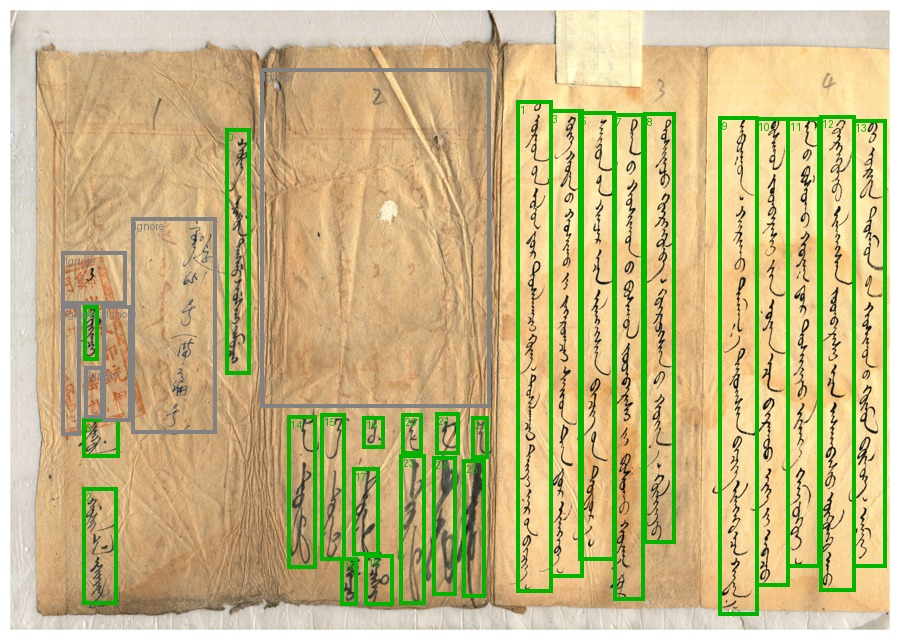
\includegraphics[width=0.75\linewidth]{figures/page_layout_annotation_example.jpg}
\caption{Example of the page-level annotation protocol. Green boxes indicate valid text columns with reading-order indices, while gray boxes indicate ignored regions that should not be counted as false positives.}
\label{fig:annotation}
\end{figure}

\section{Method}
\subsection{Rule-Based Baseline}
We evaluate three non-deep baselines before introducing YOLOv8n. The Sauvola-projection baseline applies local thresholding followed by vertical projection valley detection. The connected-component baseline groups foreground components into candidate column regions. The stronger rule-based baseline uses binarization, projection statistics, connected components, and heuristic filtering to identify vertical text-column candidates. The image is first converted to grayscale and binarized with an adaptive threshold. Vertical ink-density projections are then computed to obtain candidate column intervals. Connected components are used to suppress isolated stains and to estimate the vertical extent of each candidate. Finally, candidates are filtered by width, height coverage, and ink density, and overlapping candidates are merged before assigning a left-to-right reading order. This baseline is interpretable and does not require training data, but it is sensitive to paper noise, faint ink, and long-column over-merging. In the released code, all thresholds are fixed before test evaluation and the same ignore-region filtering protocol is used for both rule-based and learning-based predictions.

\subsection{YOLOv8n Column Detector}
We train a lightweight YOLOv8n detector~\cite{jocher2023yolov8} on page-level column boxes. YOLOv8n is selected as a practical baseline because it is fast, widely reproducible, and suitable for small custom detection datasets. The final detector is initialized from the public YOLOv8n weights and trained for 50 epochs with image size 960 and batch size 1. A batch size of 1 is used because full-page archive images are high resolution and the project was trained under limited local compute. The validation split is used only to select the confidence threshold. The main reported setting uses threshold 0.35, which gives the best validation F1 under the project-level IoU@0.5 matching metric. We do not claim architectural novelty in the detector itself; the methodological contribution of this version is the page-level annotation protocol, rotation-aware ordering, and transcript-free evaluation setting for traditional Mongolian archival pages.


\subsection{Column-Aware Post-processing Diagnostic}
To test whether explicit vertical-column priors improve detection, we additionally evaluate a simple column-aware post-processing variant for YOLO predictions. Candidate boxes are retained only if they satisfy validation-selected geometric constraints on confidence, aspect ratio, relative height, and relative width. Specifically, for a box with width $w$, height $h$, page width $W$, and page height $H$, the diagnostic filter keeps boxes satisfying $s\geq\theta$, $h/w\geq a_{\min}$, $h/H\geq r_h$, and $r_{w,\min}\leq w/W\leq r_{w,\max}$. The parameters are selected on the validation split by F1. This module is not used as the main result because the small validation set makes hand-tuned geometry priors prone to overfitting; it is included to clarify the trade-off between column priors, recall, and reading-order robustness.

\subsection{Faster R-CNN Detector Baseline}
To address the need for a stronger detector comparison, we additionally fine-tune a Faster R-CNN MobileNetV3-FPN detector initialized from COCO-pretrained weights. The classification head is replaced with a two-class head for background and TextColumn. We fine-tune for 5 epochs with learning rate 0.0005 and image max-side 960. The confidence threshold is selected on the validation split, where 0.8 gives the best F1, and the selected threshold is then applied unchanged to the test split. This baseline provides a two-stage detector comparison against the one-stage YOLOv8n detector.

\subsection{Document-Layout Detector Transfer Baselines}
We also examine two additional transfer baselines that are commonly associated with modern document-layout detection: RT-DETR and DocLayout-YOLO. RT-DETR is initialized from public pretrained weights and fine-tuned for 5 epochs at image size 640 under the same train/validation/test split. DocLayout-YOLO is initialized from a DocStructBench-pretrained checkpoint and fine-tuned for 5 epochs at image size 1024. For both baselines, the confidence threshold is selected only on the validation split before test evaluation. These models are included as supplementary transfer baselines because their pretraining domains are dominated by modern printed document layouts, which differ substantially from sparse, vertical, handwritten, and degraded archival columns. Because their training budgets are not identical to YOLOv8n, we treat them as diagnostic transfer experiments rather than fully optimized head-to-head comparisons.


\subsection{Training-Budget and Threshold Protocol}
Table~\ref{tab:training_protocol} summarizes the training and threshold-selection protocol. The primary learned comparison is between YOLOv8n and Faster R-CNN, both initialized from generic object-detection weights and adapted to the TextColumn class. RT-DETR and DocLayout-YOLO are reported separately to test whether modern document-layout priors transfer directly to this archive domain. All fixed-threshold test results use a threshold selected on the validation split, and no threshold is tuned on the test set.

\begin{table}[t]
\centering
\caption{Training-budget and threshold-selection protocol. Transfer baselines are diagnostic rather than fully optimized comparisons because their architectures and pretraining domains differ substantially.}
\label{tab:training_protocol}
\resizebox{\linewidth}{!}{%
\begin{tabular}{lcccl}
\toprule
Model & Init. domain & Epochs & Image size & Test threshold source \\
\midrule
YOLOv8n & COCO/general detection & 50 & 960 & validation F1, threshold 0.35 \\
Faster R-CNN MobileNetV3-FPN & COCO/general detection & 5 & 960 max-side & validation F1, threshold 0.80 \\
RT-DETR-L & general detection & 5 & 640 & validation F1, threshold 0.10 \\
DocLayout-YOLO & DocStructBench layout & 5 & 1024 & validation F1, threshold 0.03 \\
\bottomrule
\end{tabular}%
}
\end{table}

\subsection{Rotation-Aware Reading-Order Recovery}
YOLO detections are unordered. For ordinary pages, detections are sorted by column center from left to right. For pages relabeled after 90-degree rotation, the order is reversed. Formally, for detections $b_i=(x_{1i},y_{1i},x_{2i},y_{2i})$, the column center is $c_i=(x_{1i}+x_{2i})/2$; detections are sorted by $c_i$ ascending for ordinary pages and descending for rotated pages. This step changes only the reading-order field and does not modify detection boxes. The rule is intentionally simple and transparent, and its limitations on multi-block or irregular layouts are discussed in Section~\ref{sec:discussion}.

\subsection{Crop-Export Interface}
The pipeline exports both oracle crops from ground-truth boxes and detected crops from YOLO boxes. These crops can be passed to an existing OCR recognizer. However, because no expert column-level transcripts are currently available, CER/WER is not reported in this paper.

\section{Experiments}
\subsection{Evaluation Metrics}
Column detection is evaluated with greedy IoU@0.5 matching. Given true positives $TP$, false positives $FP$, and false negatives $FN$, we compute $P=TP/(TP+FP)$, $R=TP/(TP+FN)$, and $F1=2TP/(2TP+FP+FN)$. Mean IoU is averaged over matched prediction--ground-truth pairs. Reading-order accuracy is pairwise: for every pair of matched columns, we check whether the relative order of the two predictions is consistent with the relative order of their matched ground-truth columns. Predictions substantially overlapping ignored regions are not counted as false positives. In response to the strict page-level nature of archival processing, we also report complete detection rate, full-page success rate, Kendall's $\tau$, Spearman's $\rho$, and stratified performance by page type. Complete detection requires all valid columns on a page to be matched with no false positives or false negatives; full-page success additionally requires perfect matched-pair reading order. To quantify the uncertainty caused by the small test set, we perform page-level bootstrap resampling with 1000 samples and report 95\% confidence intervals for P/R/F1.

\subsection{Main Results}
\begin{table}[t]
\centering
\caption{Unified test-set comparison under IoU@0.5 matching. RO Acc. denotes reading-order accuracy.}
\label{tab:main_results}
\resizebox{\linewidth}{!}{%
\begin{tabular}{lccccc}
\toprule
Method & Prec. & Rec. & F1 & Mean IoU & RO Acc. \\
\midrule
Sauvola + projection & 0.344 & 0.276 & 0.307 & 0.644 & 1.000 \\
Connected components & 0.109 & 0.033 & 0.051 & 0.600 & -- \\
Heuristic column extraction & 0.436 & 0.605 & 0.507 & \textbf{0.826} & 0.900 \\
YOLOv8n + rotation-aware order & \textbf{0.956} & 0.717 & 0.820 & 0.770 & \textbf{0.900} \\
Faster R-CNN MobileNet + rotation-aware order & 0.912 & \textbf{0.750} & \textbf{0.823} & 0.738 & 0.818 \\
\bottomrule
\end{tabular}%
}
\end{table}

Table~\ref{tab:main_results} compares two classical baselines, the improved rule-based pipeline, and two learning-based detectors. The simple Sauvola-projection baseline obtains high order accuracy only on the few matched boxes, but misses most columns. Connected components performs poorly because stains, broken strokes, and large handwriting components do not correspond to complete vertical text columns. The heuristic column-extraction pipeline is substantially stronger than these classical baselines, while both learned detectors further improve precision, recall, and F1. Faster R-CNN obtains the highest F1 in this setting, whereas YOLOv8n achieves the highest reading-order accuracy and slightly higher precision. The rule-based method has a higher mean IoU on successfully matched boxes, but its recall is much lower because degraded and short columns are often missed. To make the fixed-threshold evaluation auditable, Table~\ref{tab:main_counts} reports the underlying TP/FP/FN counts used to compute the main metrics.

\begin{table}[t]
\centering
\caption{Raw detection counts for the main test-set comparison. All methods are evaluated against 152 non-ignored ground-truth text columns.}
\label{tab:main_counts}
\begin{tabular}{lrrrr}
\toprule
Method & Pred. & TP & FP & FN \\
\midrule
Sauvola + projection & 122 & 42 & 80 & 110 \\
Connected components & 46 & 5 & 41 & 147 \\
Heuristic column extraction & 211 & 92 & 119 & 60 \\
YOLOv8n + rotation-aware order & 114 & 109 & 5 & 43 \\
Faster R-CNN MobileNet + rotation-aware order & 125 & 114 & 11 & 38 \\
\bottomrule
\end{tabular}
\end{table}

\begin{table}[t]
\centering
\caption{Supplementary page-level and reading-order metrics on the test split. Complete detection requires zero false positives and zero false negatives on a page; full-page success additionally requires perfect reading order among matched columns.}
\label{tab:enhanced_order}
\resizebox{\linewidth}{!}{%
\begin{tabular}{lcccc}
\toprule
Method & Complete det. & Full-page success & Kendall $\tau$ & Spearman $\rho$ \\
\midrule
Heuristic column extraction & 0.000 & 0.000 & 0.800 & 0.796 \\
YOLOv8n + rotation-aware order & 0.000 & 0.000 & \textbf{0.800} & 0.797 \\
\bottomrule
\end{tabular}%
}
\end{table}

The strict page-level metrics in Table~\ref{tab:enhanced_order} are intentionally more demanding than box-level F1. Neither method fully solves every page, because even one missed column or one extra column makes complete detection fail. However, the matched-order correlations remain high, indicating that the remaining difficulty is dominated more by missed columns and boundary decisions than by global order reversal after the rotation-aware rule is applied.

\begin{table}[t]
\centering
\caption{Stratified YOLOv8n test performance under IoU@0.5. These groups are not mutually exclusive; they diagnose sensitivity to page complexity, orientation, and ignored regions.}
\label{tab:stratified_yolo}
\begin{tabular}{lcccc}
\toprule
Group & Pages & Prec. & Rec. & F1 \\
\midrule
Few columns ($\leq$5) & 1 & 0.000 & 0.000 & 0.000 \\
Medium columns (6--15) & 5 & 0.943 & 0.579 & 0.717 \\
Many columns ($>$15) & 5 & 0.908 & 0.663 & 0.767 \\
Rotated pages & 2 & \textbf{1.000} & 0.357 & 0.526 \\
Pages with Ignore regions & 10 & 0.910 & 0.574 & 0.704 \\
No-Ignore page & 1 & 0.955 & \textbf{0.955} & \textbf{0.955} \\
\bottomrule
\end{tabular}
\end{table}

Table~\ref{tab:stratified_yolo} provides diagnostic observations rather than statistically stable subgroup conclusions, because several groups contain only one or two pages. The detector performs best on the no-ignore page and remains reasonably strong on many-column pages, but it is weak on the single few-column test page and recall drops on rotated pages. This supports the failure analysis that fixed confidence thresholds and orientation-specific cases remain important targets for future improvement.

\begin{table}[t]
\centering
\caption{Supplementary transfer-detector baselines under the same validation-selected threshold protocol. These negative results suggest that off-the-shelf modern document-layout priors transfer poorly to sparse vertical handwritten archive columns without stronger domain adaptation.}
\label{tab:transfer_baselines}
\begin{tabular}{lccccc}
\toprule
Method & Prec. & Rec. & F1 & Mean IoU & RO Acc. \\
\midrule
RT-DETR-L + rotation-aware order & 0.032 & 0.270 & 0.058 & 0.632 & 0.847 \\
DocLayout-YOLO + rotation-aware order & 0.046 & 0.031 & 0.037 & 0.572 & 0.000 \\
\bottomrule
\end{tabular}
\end{table}

Table~\ref{tab:transfer_baselines} reports two additional detector-transfer attempts. Both perform much worse than the task-specific YOLOv8n and Faster R-CNN baselines. The main failure mode is a large number of low-quality candidate regions or a mismatch between modern layout categories and the target TextColumn unit. Because these models were not trained with the same budget as YOLOv8n, we interpret them conservatively as diagnostic evidence of non-trivial domain transfer rather than as definitive model rankings.


\begin{table}[t]
\centering
\caption{Supplementary strict-localization comparison at IoU@0.75. Compared with Table~\ref{tab:main_results}, the stricter threshold penalizes boundary errors more heavily.}
\label{tab:iou75}
\resizebox{\linewidth}{!}{%
\begin{tabular}{lccccc}
\toprule
Method & Prec. & Rec. & F1 & Mean IoU & RO Acc. \\
\midrule
Heuristic column extraction & 0.322 & 0.447 & 0.375 & \textbf{0.901} & \textbf{1.000} \\
YOLOv8n + rotation-aware order & \textbf{0.579} & \textbf{0.434} & \textbf{0.496} & 0.826 & \textbf{1.000} \\
Faster R-CNN MobileNet + rotation-aware order & 0.352 & 0.289 & 0.318 & 0.828 & \textbf{1.000} \\
\bottomrule
\end{tabular}%
}
\end{table}


\begin{table}[t]
\centering
\caption{Page-level bootstrap 95\% confidence intervals on the 11-page test split.}
\label{tab:bootstrap_ci}
\resizebox{\linewidth}{!}{%
\begin{tabular}{lccc}
\toprule
Method & Precision 95\% CI & Recall 95\% CI & F1 95\% CI \\
\midrule
Heuristic column extraction & [0.280, 0.611] & [0.488, 0.710] & [0.360, 0.647] \\
YOLOv8n + rotation-aware order & [0.821, 0.979] & [0.468, 0.792] & [0.601, 0.866] \\
Faster R-CNN MobileNet + rotation-aware order & [0.867, 0.958] & [0.568, 0.820] & [0.689, 0.879] \\
\bottomrule
\end{tabular}%
}
\end{table}


\subsection{Effect of Training Set Size}
We also monitored YOLOv8n performance as additional page-level annotations were added. Table~\ref{tab:train_size} reports project-level test metrics under the same IoU@0.5 matching protocol used elsewhere in this paper. Increasing the training set from 7 to 43 pages improves test recall from 0.388 to 0.717 and F1 from 0.532 to 0.820, confirming that even moderate additional layout annotation substantially improves generalization.

\begin{table}[t]
\centering
\caption{YOLOv8n project-level test performance with different numbers of annotated training pages. These metrics use the same IoU@0.5 matching protocol as Table~\ref{tab:main_results}.}
\label{tab:train_size}
\begin{tabular}{lccccc}
\toprule
Training pages & Test Prec. & Test Rec. & Test F1 & Mean IoU & RO Acc. \\
\midrule
7 & 0.843 & 0.388 & 0.532 & 0.719 & 1.000 \\
20 & 0.875 & 0.691 & 0.772 & 0.748 & 0.900 \\
43 & \textbf{0.956} & \textbf{0.717} & \textbf{0.820} & \textbf{0.770} & \textbf{0.900} \\
\bottomrule
\end{tabular}
\end{table}

\subsection{Threshold Sensitivity}
\begin{table}[t]
\centering
\caption{Validation threshold sensitivity for YOLOv8n. The final threshold is selected on the validation split, not on the test split.}
\label{tab:threshold}
\begin{tabular}{lccc}
\toprule
Threshold & Val Prec. & Val Rec. & Val F1 \\
\midrule
0.25 & 0.746 & 0.787 & 0.766 \\
0.30 & 0.812 & 0.759 & 0.785 \\
0.35 & \textbf{0.876} & 0.722 & \textbf{0.792} \\
0.40 & 0.873 & 0.639 & 0.738 \\
\bottomrule
\end{tabular}
\end{table}


\begin{table}[t]
\centering
\caption{Approximate project-level confidence-sweep AP on the test split. AP is computed by sweeping the confidence threshold over project-level predictions and applying the same ignore-region filtering protocol.}
\label{tab:project_ap}
\begin{tabular}{lcc}
\toprule
Method & AP@0.50 & AP@0.75 \\
\midrule
YOLOv8n + rotation-aware order & \textbf{0.921} & \textbf{0.399} \\
Faster R-CNN MobileNet + rotation-aware order & 0.700 & 0.097 \\
\bottomrule
\end{tabular}
\end{table}



\begin{table}[t]
\centering
\caption{Diagnostic column-aware YOLO post-processing. The parameters are selected on validation F1. The result is not used as the main setting because it improves validation F1 but reduces test recall, illustrating overfitting risk from hand-tuned geometric priors.}
\label{tab:column_aware_diag}
\resizebox{\linewidth}{!}{%
\begin{tabular}{lcccccc}
\toprule
Setting & Split & Prec. & Rec. & F1 & Mean IoU & RO Acc. \\
\midrule
Main YOLO threshold 0.35 & test & 0.956 & 0.717 & 0.820 & 0.770 & 0.900 \\
Recall-oriented threshold 0.30 & test & 0.894 & 0.675 & \textbf{0.769} & 0.760 & 0.830 \\
Column-aware prior filter & val & \textbf{0.940} & 0.722 & 0.817 & 0.784 & 0.821 \\
Column-aware prior filter & test & 0.949 & 0.730 & 0.825 & 0.760 & \textbf{0.818} \\
\bottomrule
\end{tabular}%
}
\end{table}

Table~\ref{tab:column_aware_diag} shows that explicit vertical-column priors can improve validation F1 and test reading-order accuracy, but they reduce test recall and F1. We therefore keep the simpler validation-selected YOLO threshold as the main setting and treat column-aware filtering as a diagnostic experiment rather than a claimed improvement. This negative result is useful because it indicates that future column-aware modeling should be learned or regularized more robustly instead of relying only on hand-tuned geometric thresholds.

\subsection{Qualitative Analysis}
\begin{figure}[t]
\centering
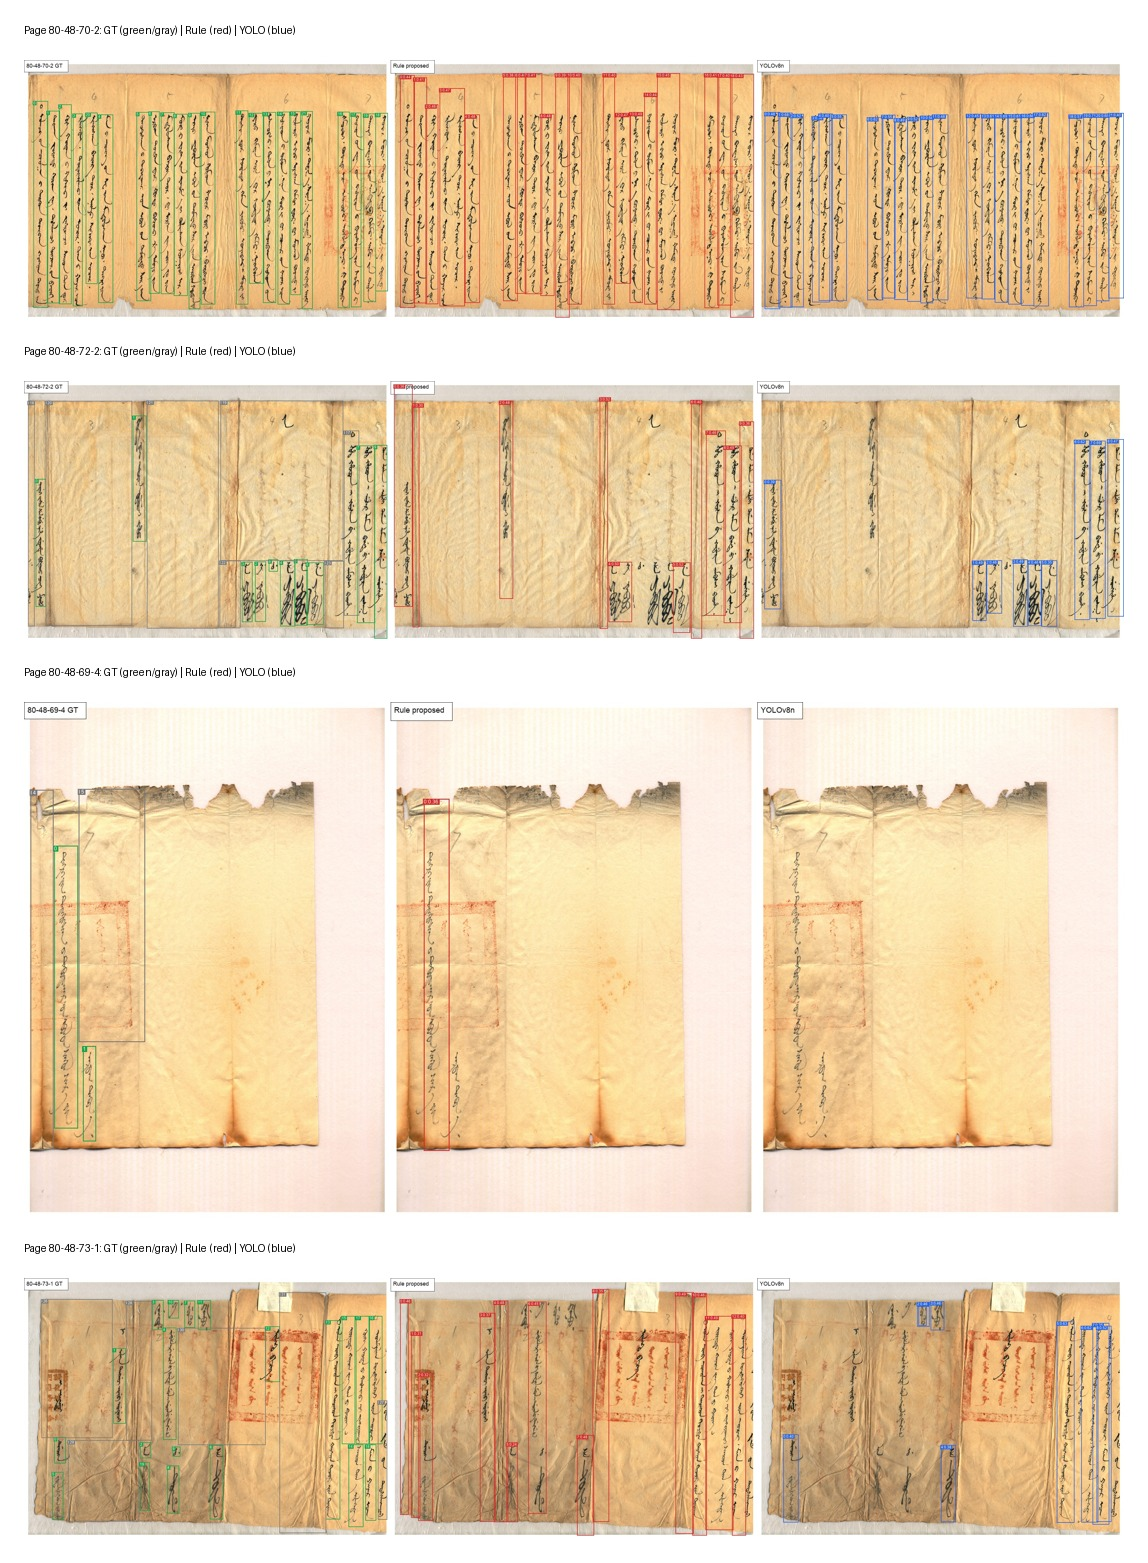
\includegraphics[width=0.88\linewidth]{figures/page_layout_qualitative_failure_montage.jpg}
\caption{Representative page-level comparisons. Each row shows ground truth, rule-based predictions, and YOLOv8n predictions. Green denotes valid text columns, gray denotes ignored regions, red denotes rule-based detections, and blue denotes YOLO detections.}
\label{fig:qualitative}
\end{figure}

The qualitative examples show that YOLOv8n reduces many false columns caused by noise and page borders, while also recovering more degraded columns than the rule-based method. Remaining errors are concentrated on few-column pages, pages with severe over-merging, and ambiguous noisy regions.




\subsection{Ablation of Ignore Filtering and Rotation-Aware Ordering}
Table~\ref{tab:ablation} evaluates two post-processing choices at the selected confidence threshold 0.35. On the corrected test labels, ignore-region filtering does not suppress any YOLO predictions, so detection F1 is unchanged across the four settings. Rotation-aware ordering also leaves detection F1 unchanged, but on this small test split the x-sorted order happens to give slightly higher reading-order accuracy than the rotation-aware heuristic. This means the ordering rule should still be treated as a diagnostic heuristic rather than a fully solved component.

\begin{table}[t]
\centering
\caption{Ablation of ignore-region filtering and rotation-aware reading order at score threshold 0.35. Removed denotes predictions suppressed because they overlap an Ignore region.}
\label{tab:ablation}
\resizebox{\linewidth}{!}{%
\begin{tabular}{lcccccc}
\toprule
Configuration & Prec. & Rec. & F1 & RO Acc. & FP/FN & Removed \\
\midrule
Full: ignore + rotation-aware order & \textbf{0.956} & 0.717 & \textbf{0.820} & 0.900 & 5 / 43 & 0 \\
w/o rotation-aware order & \textbf{0.956} & 0.717 & \textbf{0.820} & \textbf{1.000} & 5 / 43 & 0 \\
w/o ignore filtering & \textbf{0.956} & 0.717 & \textbf{0.820} & 0.900 & 5 / 43 & 0 \\
w/o both & \textbf{0.956} & 0.717 & \textbf{0.820} & \textbf{1.000} & 5 / 43 & 0 \\
\bottomrule
\end{tabular}%
}
\end{table}


\subsection{Inference-Size Sensitivity}
To partially examine the effect of image resolution without retraining the detector, we run the same YOLOv8n checkpoint with three inference sizes on the test split. Table~\ref{tab:imgsz_ablation} shows that 640 is faster but misses many columns, while 1280 increases recall but also introduces more false positives and higher runtime compared with 960. The selected 960 setting is aligned with the main project-level evaluation protocol and offers the best F1-speed balance in this local CPU evaluation.

\begin{table}[t]
\centering
\caption{Inference-size sensitivity using the same trained YOLOv8n checkpoint and score threshold 0.35. This is an inference-only ablation, not a retraining experiment.}
\label{tab:imgsz_ablation}
\begin{tabular}{lcccccc}
\toprule
imgsz & Prec. & Rec. & F1 & Mean IoU & RO Acc. & Mean s/page \\
\midrule
640 & 0.888 & 0.485 & 0.627 & 0.779 & 0.932 & \textbf{0.182} \\
960 & \textbf{0.914} & 0.650 & \textbf{0.760} & 0.773 & 0.931 & 0.252 \\
1280 & 0.773 & \textbf{0.669} & 0.717 & 0.766 & \textbf{0.947} & 0.489 \\
\bottomrule
\end{tabular}
\end{table}

\subsection{Runtime Analysis}
We measure inference time on the 11-page test split using local CPU execution. The rule-based pipeline requires 1.84 seconds per page on average, while YOLOv8n requires 0.19 seconds per page at image size 960 after a one-image warm-up. These measurements indicate that the learning-based detector is not only more accurate under the main metric, but also faster in the current implementation.

\begin{table}[t]
\centering
\caption{Runtime on the 11-page test split under local CPU execution.}
\label{tab:runtime}
\resizebox{\linewidth}{!}{%
\begin{tabular}{lccc}
\toprule
Method & Device & Mean s/page & Median s/page \\
\midrule
Heuristic column extraction & CPU & 1.843 & 1.729 \\
YOLOv8n + rotation-aware order & CPU & 0.193 & 0.196 \\
Faster R-CNN MobileNet + rotation-aware order & CPU & \textbf{0.168} & \textbf{0.162} \\
\bottomrule
\end{tabular}%
}
\end{table}

\subsection{Failure Analysis}
The remaining errors can be grouped into five categories. First, few-column pages are sensitive to a fixed confidence threshold; for example, some valid columns may be filtered out at threshold 0.35. Second, rule-based methods tend to over-merge multiple short text segments into long boxes, producing simultaneous false positives and false negatives under IoU matching. Third, rotated or upside-down scans require explicit orientation handling, otherwise the box order may be geometrically valid but semantically reversed. Fourth, red seals, paper stains, and edge shadows still introduce ambiguous regions that require either ignore annotations or stronger artifact modeling. Fifth, the diagnostic column-aware post-processing in Table~\ref{tab:column_aware_diag} shows that hand-tuned vertical-column priors can overfit validation statistics and reduce test recall, motivating learned or data-adaptive column priors in future work.

\section{Discussion and Limitations}
\label{sec:discussion}
This study intentionally focuses on layout analysis rather than transcription-based OCR accuracy. To assess annotation reliability, we also asked an independent annotator to label a 5-page subset. The resulting agreement is moderate to strong for text-column boxes (F1@0.5 = 0.852) and mean matched IoU (0.800), while reading-order agreement is lower (0.677), reflecting the ambiguity of some multi-column pages. Ignore-region agreement remains weaker and is now explicitly treated as a limitation rather than a polished result; the refined Ignore subtypes in Table~\ref{tab:ignore_subtypes} are intended to improve future annotation consistency. Since expert transcription of handwritten traditional Mongolian columns is unavailable, reporting CER/WER would be misleading. The current pipeline is nevertheless crop-export-ready: it can export oracle and automatically detected column crops and connect them to a recognizer once reliable transcripts are added.

Important limitations remain. A fixed confidence threshold can miss few-column pages; rule-based post-processing may over-merge multi-segment columns; and pages with seals or strong background noise still require more robust artifact handling. Ignore-region agreement in the 5-page IAA subset is lower than box agreement, suggesting that even the refined Ignore subtype guideline requires more examples and annotator training before it can be considered mature. The project-level AP results in Table~\ref{tab:project_ap} and the stricter IoU@0.75 results in Table~\ref{tab:iou75} show that boundary precision remains challenging, especially under high-overlap evaluation. The current test split is also small, so the bootstrap intervals in Table~\ref{tab:bootstrap_ci} should be interpreted as an honest uncertainty estimate rather than a final large-scale benchmark. The transfer baselines in Table~\ref{tab:transfer_baselines} also suggest that modern document-layout detectors do not automatically solve this historical archive setting, but the unequal training budgets in Table~\ref{tab:training_protocol} mean that these results should be interpreted as diagnostic transfer tests rather than final optimized comparisons; stronger domain adaptation, column-aware pretraining, and fairer compute-matched retraining remain necessary. Faster R-CNN was not exhaustively optimized in this study; its strong IoU@0.5 result suggests that two-stage detection deserves further investigation under a compute-matched protocol. Future work will add a small expert-transcribed subset, enabling oracle-crop and detected-crop CER/WER evaluation. The inference-size sensitivity in Table~\ref{tab:imgsz_ablation} is only an inference-only ablation; full retraining at different image sizes remains future work.

\section{Conclusion}
We presented a pilot-scale page-level layout-analysis benchmark for traditional Mongolian historical archives under a realistic low-resource condition where expert text transcription is unavailable. By shifting the evaluation focus to text-column detection and reading-order recovery, the proposed workflow provides an initial benchmark and a partially reproducible crop-export interface for future archival OCR. Learning-based detectors with rotation-aware reading-order recovery substantially outperform the heuristic baseline on the independent test split. YOLOv8n achieves 0.820 F1 and 0.900 reading-order accuracy, while Faster R-CNN MobileNet achieves 0.823 F1 after COCO-pretrained fine-tuning. However, the complete detection rate and full-page success rate are still 0 on the current test split; therefore the present system should be viewed as a candidate crop generator rather than a fully automatic page-level OCR preprocessing solution.


\section*{Data Availability}
The current project materials include the annotation schema, page-level annotation files, split manifests, evaluation scripts, trained-detector configuration notes, and generated prediction files. These non-image research artifacts can be shared with reviewers or released publicly when allowed by project policy. The archive images themselves are subject to institutional access constraints and should be released only according to archive data-sharing policy. Complete end-to-end reproduction therefore requires authorized access to the original archive images, while metric computation can be reproduced from the shared annotations and prediction files.

\section*{Author Contributions}
Lanying Liang: Conceptualization, Data Curation, Writing -- Original Draft. Yuefeng Liu: Methodology, Software, Validation, Writing -- Review \& Editing, Supervision.

\section*{Ethics Statement}
This study uses historical archive images for document analysis and digital preservation. No personal intervention or modern human-subject experiment is involved. The work does not attempt to infer sensitive attributes of living individuals.

\section*{Funding}
This work was supported by the National Natural Science Foundation of China (Grant No. 62341604), the Science and Technology Project of Inner Mongolia Autonomous Region Archives Bureau (Grant No. 2022-36), the China Scholarship Council (Grant No. 202408150080), and the General Project of the 14th Five-Year Plan for Educational Science of Inner Mongolia Autonomous Region (Grant No. NGJGH2025013).


\begin{thebibliography}{10}

\bibitem{likforman2007textline}
L. Likforman-Sulem, A. Zahour, and B. Taconet, ``Text line segmentation of historical documents: a survey,'' \emph{International Journal on Document Analysis and Recognition}, vol. 9, pp. 123--138, 2007. doi: 10.1007/s10032-006-0023-z.

\bibitem{nikolaidou2022survey}
K. Nikolaidou, M. Seuret, H. Mokayed, and M. Liwicki, ``A survey of historical document image datasets,'' \emph{International Journal on Document Analysis and Recognition}, vol. 25, pp. 305--338, 2022. doi: 10.1007/s10032-022-00405-8.

\bibitem{gruning2017readbad}
T. Gr\"uning, R. Labahn, M. Diem, F. Kleber, and S. Fiel, ``READ-BAD: A new dataset and evaluation scheme for baseline detection in archival documents,'' arXiv:1705.03311, 2017.

\bibitem{zhong2019publaynet}
X. Zhong, J. Tang, and A. J. Yepes, ``PubLayNet: largest dataset ever for document layout analysis,'' in \emph{Proc. International Conference on Document Analysis and Recognition}, 2019, pp. 1015--1022. doi: 10.1109/ICDAR.2019.00166.

\bibitem{pfitzmann2022doclaynet}
B. Pfitzmann, C. Auer, M. Dolfi, A. S. Nassar, and P. W. J. Staar, ``DocLayNet: A large human-annotated dataset for document-layout analysis,'' in \emph{Proc. ACM SIGKDD International Conference on Knowledge Discovery and Data Mining}, 2022. doi: 10.1145/3534678.3539043.

\bibitem{shen2021layoutparser}
Z. Shen, R. Zhang, M. Dell, B. C. G. Lee, J. Carlson, and W. Li, ``LayoutParser: A unified toolkit for deep learning based document image analysis,'' in \emph{Document Analysis and Recognition -- ICDAR 2021}, LNCS 12821, pp. 131--146, 2021. doi: 10.1007/978-3-030-86549-8\_9.

\bibitem{quiros2022reading}
L. Quir\'os and E. Vidal, ``Reading order detection on handwritten documents,'' \emph{Neural Computing and Applications}, vol. 34, pp. 9593--9611, 2022. doi: 10.1007/s00521-022-06948-5.

\bibitem{neudecker2019ocrd}
C. Neudecker, K. Baierer, M. Federbusch, M. Boenig, K.-M. W\"urzner, V. Hartmann, and E. Herrmann, ``OCR-D: An end-to-end open source OCR framework for historical printed documents,'' in \emph{Proc. DATeCH2019}, 2019, pp. 53--58. doi: 10.1145/3322905.3322917.


\bibitem{pan2023molhw}
Y. Pan, D. Fan, H. Wu, and D. Teng, ``A new dataset for Mongolian online handwritten recognition,'' \emph{Scientific Reports}, vol. 13, article 26, 2023. doi: 10.1038/s41598-022-27267-8.

\bibitem{deng2023yolo}
Q. Deng, M. Ibrayim, A. Hamdulla, and C. Zhang, ``The YOLO model that still excels in document layout analysis,'' \emph{Signal, Image and Video Processing}, vol. 18, no. 2, pp. 1539--1548, 2024. doi: 10.1007/s11760-023-02838-y.

\bibitem{zhao2024doclayout}
Z. Zhao, H. Kang, B. Wang, and C. He, ``DocLayout-YOLO: Enhancing document layout analysis through diverse synthetic data and global-to-local adaptive perception,'' arXiv:2410.12628, 2024.

\bibitem{jocher2023yolov8}
G. Jocher, A. Chaurasia, and J. Qiu, ``Ultralytics YOLOv8,'' software, version 8.0.0, 2023. Available: \url{https://github.com/ultralytics/ultralytics}.

\end{thebibliography}

\end{document}
